\documentclass[border=2pt]{standalone}

%% Fonts
%\usepackage{fontspec}
%% Default Features
%\defaultfontfeatures{
%	Mapping=tex-text,
%	Ligatures=TeX,
%}
%% Serif Font
%\setmainfont[
%	UprightFont=EBGaramond-Regular,
%	ItalicFont=EBGaramond-Italic,
%	BoldFont=EBGaramond-Bold,
%	BoldItalicFont=EBGaramond-BoldItalic,
%]{EB Garamond}
%% Mono Font
%\setmonofont[
%	UprightFont=JetBrainsMonoNL-Regular,
%	ItalicFont=JetBrainsMonoNL-Italic,
%	BoldFont=JetBrainsMonoNL-Bold,
%	BoldItalicFont=JetBrainsMonoNL-BoldItalic,
%]
%{JetBrains Mono}

% Tikz
\usepackage{tikz}
\usetikzlibrary{calc, positioning, shapes}

% Colors
%\definecolor{myyellow}{RGB}{255, 255, 191}
%\definecolor{mygreen}{RGB}{171, 221, 164}
%\definecolor{myblue}{RGB}{216, 225, 246}
% Dimensions
\def\deltadim{0.1}
\def\cornerradius{0.2cm}
\def\innersep{6pt}
\def\outersep{2pt}
% Threads
\def\threaddrawcolor{yellow!60!black}
\def\threadfillcolor{yellow!20}
\def\shift{1cm}
%% Peer threads
\def\numpeerthreads{4}
%% Service Threads
\def\numservicethreads{3}
%% Timer Threads
\def\numtimerthreads{2}
% Consensus State
\def\consensusstatedrawcolor{green!70!black}
\def\consensusstatefillcolor{green!20}
\def\consensusstateheight{2.25cm}
\def\consensusstatewidth{4.5cm}
% Lock
\def\lockdrawcolor{orange!50!black}
\def\lockfillcolor{orange!50}
\def\lockhandlecolor{black}
\def\locksize{12pt}
% Data Store
\def\datastoredrawcolor{orange!80!black}
\def\datastorefillcolor{orange!60}
\def\datastoreheight{6pt}
\def\datastorewidth{12pt}

% Styles
\tikzset{
	% labels
	label/.style={
		font=\small\ttfamily,
		align=center,
	},
	% node labels
	node_label/.style={
		font=\small,
		align=center,
	},
	% general
	module/.style={
		draw,
		very thick,
		label,
		outer sep=\outersep,
		rounded corners=\cornerradius,
		shape=rectangle,
	},
	% threads
	thread/.style={
		module,
		draw=\threaddrawcolor,
		fill=\threadfillcolor,
		inner xsep=\innersep,
		inner ysep=\innersep,	
	},
	% consensus state
	consensus_state/.style={
		module,
		draw=\consensusstatedrawcolor,
		fill=\consensusstatefillcolor,
		minimum height=\consensusstateheight,
		minimum width=\consensusstatewidth,
	},
	% parts of consensus state
	consensus_state_parts/.style={
		module,
		draw=\consensusstatedrawcolor,
		fill=\consensusstatefillcolor,
		inner xsep=\innersep,
		inner ysep=\innersep,
	},
	% lock
	lock_body/.style={
		draw=\lockdrawcolor,
		fill=\lockfillcolor,
		very thick,
		shape=rectangle,
		minimum size=\locksize,
		inner sep=0,
		outer sep=0,
	},
	lock_handle/.style={
		draw=black,
		very thick, 
		looseness=2
	},
	% data store
	data_store/.style={
		draw=\datastoredrawcolor,
		fill=\datastorefillcolor,
		thick,
		ellipse,
		inner sep=0,
		minimum height=\datastoreheight,
		minimum width=\datastorewidth,
	},
	% connections
	connection/.style={
		thick,
		-stealth,
	},
	% traffic
	inbound_traffic/.style={
		very thick,
		latex-,
	},
	outbound_traffic/.style={
		very thick,
		-latex,
	}
}

\begin{document}
	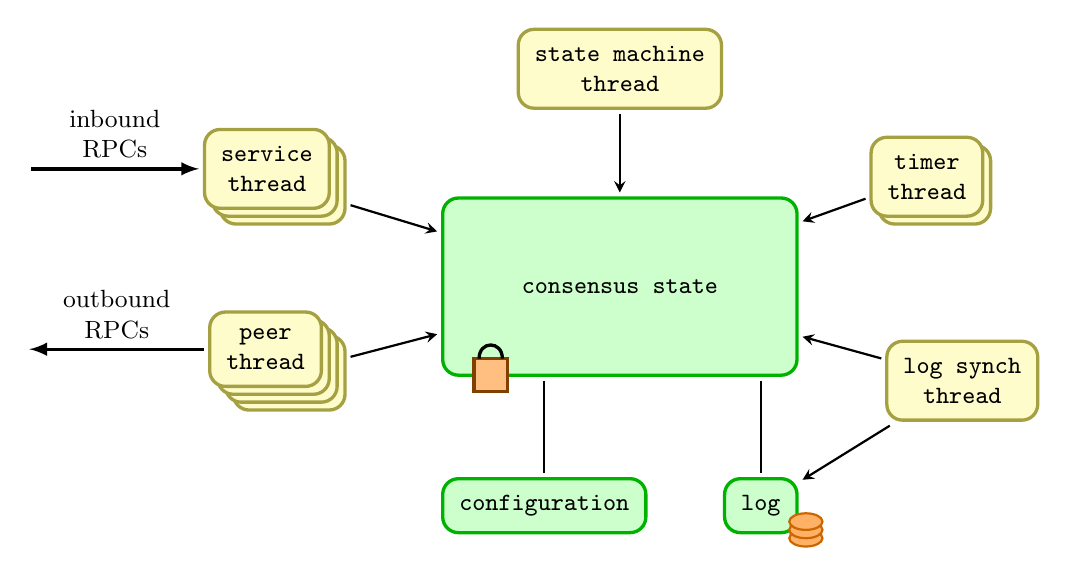
\begin{tikzpicture}
		% Consensus state
		\node [
			consensus_state,
		] (consensus state) {consensus state};
		%% Configuration
		\node [
			consensus_state_parts,
			anchor=south west,
			shift={(0,-\shift*2)},
		] (configuration) at (consensus state.south west) {configuration};
		%% Lock
		\coordinate (lock_body_x) at ($(configuration.mid)!0.5!(configuration.west)$);
		\node[
			lock_body,
			anchor=north,
			shift={(0,\outersep + \locksize/2)},
		] (lock_body) at (lock_body_x|-consensus state.south) {};
		\draw[
			lock_handle
		] (lock_body.125) to[out=90, in=90] (lock_body.55);
		%% Log
		\node [
			consensus_state_parts,
			anchor=south east,
			shift={(0,-\shift*2)},
		] (log) at (consensus state.south east) {log};
		%% Data store
		\foreach \i in {0,...,2} {
			\node[
				data_store,
				shift={(\datastorewidth/10,\i * \datastoreheight/2)},
			] at (log.south east) {};
		}	
	
		% Peer threads
		\coordinate (peer_thread) at ($(consensus state.south west) + (-\shift,0)$);
		
		\foreach \i in {1,...,\numpeerthreads} {
			\pgfmathsetmacro{\displacement}{\i * \deltadim}
			\node[
				thread,
				anchor=east
			] (peer_thread\i) at ($(peer_thread) + (-\displacement,\displacement)$) {peer\\thread};
		}

		% Service threads
		\coordinate (service_thread) at ($(consensus state.north west) + (-\shift,0)$);
		
		\foreach \i in {1,...,\numservicethreads} {
			\pgfmathsetmacro{\displacement}{\i * \deltadim}
			\node[
				thread,
				anchor=east
			] (service_thread\i) at ($(service_thread) + (-\displacement,\displacement)$) {service\\thread};
		}
		
		% State Machine
		\node[
			thread,
			anchor=south
		] (state_machine_thread) at ($(consensus state.north) + (0,\shift)$) {state machine\\thread};
		
		% Timer threads
		\coordinate (timer_thread) at ($(consensus state.north east) + (\shift,0)$);
		
		\foreach \i in {1,...,\numtimerthreads} {
			\pgfmathsetmacro{\displacement}{\i * \deltadim}
			\node[
				thread,
				anchor=west
			] (timer_thread\i) at ($(timer_thread) + (-\displacement,\displacement)$) {timer\\thread};
		}
		
		% Log synch thread
		\node[
			thread,
			anchor=west
		] (log_synch_thread) at ($(consensus state.south east) + (\shift,0)$) {log synch\\thread};
		
		% Part of
		\draw[thick] (consensus state.south-|configuration) -- (configuration);
		\draw[thick] (consensus state.south-|log) -- (log);
		
		% Traffic
		\draw[
			inbound_traffic,
			node_label
		] (service_thread\numservicethreads) 
						-- +(-\shift*3,0) 
						node[pos=0.5, above, align=center] {inbound\\RPCs};
		\draw[
			outbound_traffic,
			node_label
		] (peer_thread\numpeerthreads) 
						-- +(-\shift*3,0) 
						node[pos=0.5, above, align=center] {outbound\\RPCs};
		
		% Connections
		\draw[connection] (log_synch_thread) -- (log);
		\draw[connection] (log_synch_thread) -- (consensus state);
		\draw[connection] (timer_thread\numtimerthreads) -- (consensus state);
		\draw[connection] (state_machine_thread) -- (consensus state);		
		\draw[connection] (service_thread1) -- (consensus state);
		\draw[connection] (peer_thread1) -- (consensus state);
	\end{tikzpicture}
\end{document}